\documentclass{homework}
% \usepackage{graphicx} % Required for inserting images
\usepackage{amsmath}
\usepackage{gensymb}
\usepackage{subfig}
\usepackage{float}
\usepackage{appendix}
\usepackage{pythonhighlight}

\class{APPM 5630}
\title{Homework 6}
\author{Sean Jennings}
\date{February 28, 2025}

\begin{document}
\maketitle

\section{Problem 1}

Code which implements a gradient check is provided in \ref{sec:A1}. We implement forward and center differencing 
methods. We take the error $||\nabla f(x_0) - \tilde{\nabla} f(x0)||_2$ to be the 2-norm $\nabla$, the gradient
operator and $\tilde{\nabla}$, the numeric approximation to the gradient, at some point $x0\in \text{dom}(f)$.

For all the gradient checks, we see that the error is quite small for certain values of the stepsize, although
the optimal stepsize depends both on the finite differencing method as well as the function in question.

For example, the linear function $f(x) = ax + b$ for $a,b,x\in \R$, shown in figure \ref{fig:linear},
shows no difference between forward and central differencing. This is due to the fact that both differencing methods are
exact for a linear function. When the method is exact, the error continues to decrease as a stepsize increases since the floating
precision is the only error source. Since central differencing is accurate to the second order, we see that the central
differencing error for the 1d quadratic $f(x) = ax^2 + bx + c$ in figure \ref{fig:quad} follows a similar trend of decreasing (mostly) monotonically with stepsize,
whereas the forward differencing method begins increasing for $h>1e-8$.

\begin{center}
    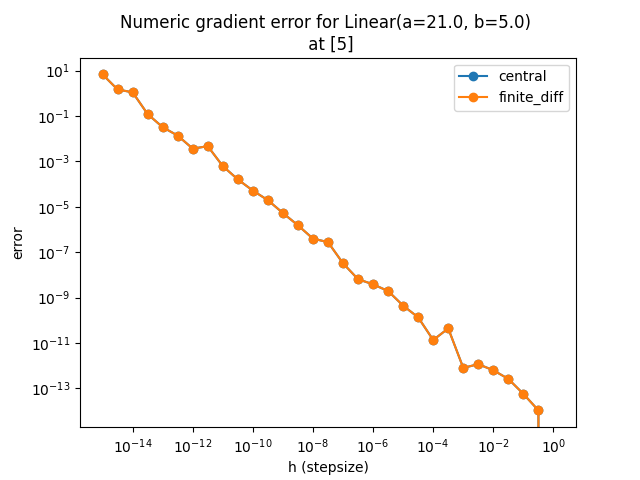
\includegraphics[width=0.6\linewidth]{Images/5_Linear(a=21.0,_b=5.0).png}
    \label{fig:linear}
    \captionof{figure}{Gradient check for linear function}
\end{center}

\begin{center}
    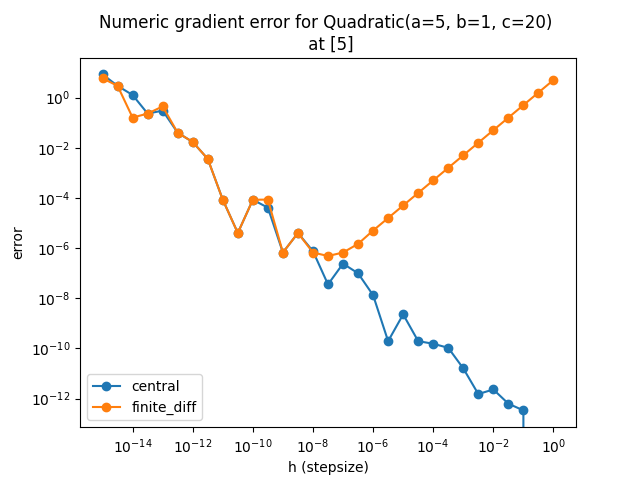
\includegraphics[width=0.6\linewidth]{Images/5_Quadratic(a=5,_b=1,_c=20).png}
    \label{fig:quad}
    \captionof{figure}{Gradient check for quadratic function}
\end{center}


Since neither method is exact for polynomials above degree 2, the cubic function
$f(x) = <c, [x^3, x^2, x, 1]^T>$ with $c\in\R^4$ (figure \ref{fig:cubic})
shows the tradeoff between decreasing approximation error (with smaller stepsize) and decreasing
floating precision error (with large stepsize) for both forward and central differencing methods.


\begin{center}
    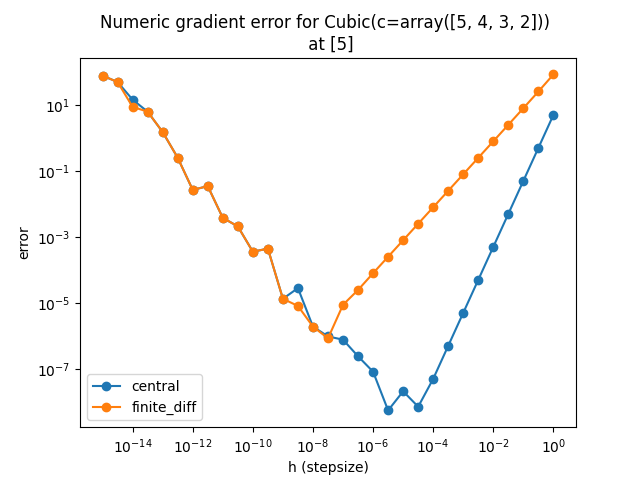
\includegraphics[width=0.6\linewidth]{Images/5_Cubic(c=array([5,_4,_3,_2])).png}
    \captionof{figure}{Gradient check for cubic function}
    \label{fig:cubic}
\end{center}

The log-likelihood of the logistic function $\ell$ (taking $X\in\R^{N\times P}$, $y\in\R^N$, $N=10$, and $P=5$) is evaluated
at two different points, a random $w_0\in\R^P$ in figure \ref{fig:log-rand-w}, and at $w_0 = 0$ in figure \ref{fig:log-zero-w}. At the random $w_0$, the gradient
check looks very similar to the linear function, implying that the sigmoid function $\sigma(-y_i w^T X_i)$ is saturated at either
0 or 1 for each $i$ and $w$ around the random $w_0$. On the other hand, at $w_0=0$ the error looks approximately quadratic.


\begin{center}
    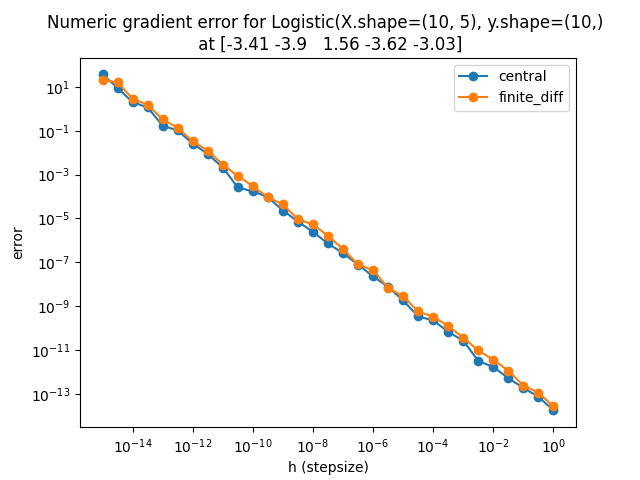
\includegraphics[width=0.6\linewidth]{Images/-3.41_Logistic(X.shape=(10,_5),_y.shape=(10,).png}
    \captionof{figure}{Gradient check log-likelihood of Logistic function and random $w_0$}
    \label{fig:log-rand-w}
\end{center}

\begin{center}
    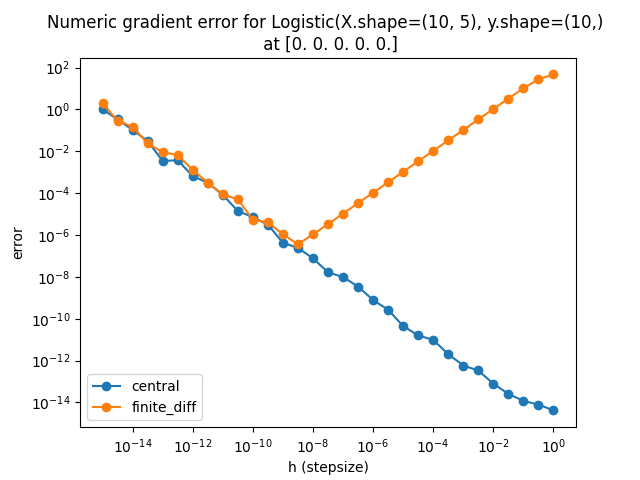
\includegraphics[width=0.6\linewidth]{Images/0.0_Logistic(X.shape=(10,_5),_y.shape=(10,).png}
    \captionof{figure}{Gradient check log-likelihood of Logistic function and $w_0=0$}
    \label{fig:log-zero-w}
\end{center}

Finally, the error for an incorrectly implemented gradient is shown in figure \ref{fig:incorrect-linear}.
The error is now approximately constant
w.r.t. the stepsize and also quite large. This gives us confidence that the logistic function and its gradient are implemented correctly.

\begin{center}
    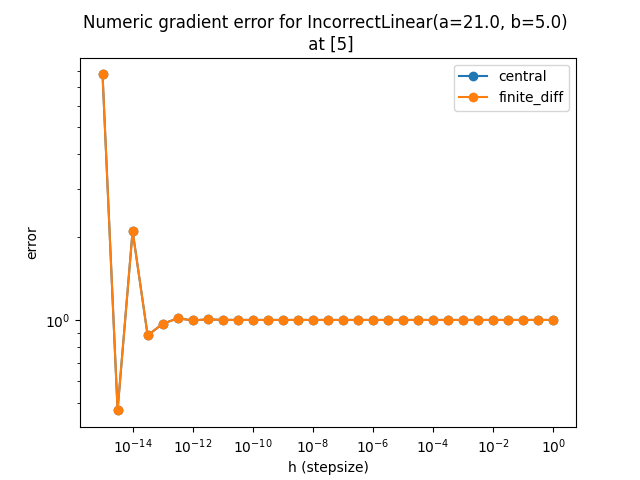
\includegraphics[width=0.6\linewidth]{Images/5_IncorrectLinear(a=21.0,_b=5.0).png}
    \captionof{figure}{Gradient check for a 1d linear function with incorrect gradient}
    \label{fig:incorrect-linear}
\end{center}

\section{Problem 2}

Code which implements gradient descent is provided in Figure \ref{fig:grad-descent}.
We test by initializing a random 100x50 matrix, and comparing our result to the one
obtained from numpy's lstsq implementation. The error over iterations is displayed in
figure \ref{fig:grad-descent-err}.

Note, code shown here evaulates $f$ twice as much as necessary (since $x_0 <- x_1$ at the end of the loop). This can
be avoided by saving function evaluations to intermediate variables, but 
we've omitted this optimization for the sake of clarity.

\begin{center}
    \begin{python}

def gradient_descent(f, grad, x0, stepsize, tol=1e-6, maxiters=int(1e3)):
    # Store iterations
    steps = np.full((maxiters, x0.shape[0]), np.nan)
    
    for i in range(maxiters):
        # Move in the descent direction
        x1 = x0 - grad(x0) * stepsize
        
        if abs(f(x1) - f(x0)) < tol:
            # Converged successfully
            return SolverResult(x1, True, steps[:i+1])
        # Update variable for next loop iteration
        x0 = x1
    # maxiters was exceeded without reaching tolerance
    return SolverResult(x0, False, steps)


# Initialize a random least-squares problem.
M = 100
N = 50
A = np.random.uniform(0, 10, (M,N))
b = np.ones(M)
x_star = np.linalg.lstsq(A, b)[0]

def f(x):
    return 1/2 * np.linalg.norm(A @ x - b)

def grad_f(x):
    return A.T @ (A @ x - b)


# And Solve.
x0 = np.zeros(N)
stepsize = 1 / spectral_norm(A)**2
res = gradient_descent(f, grad_f, x0, stepsize, tol=1e-10, maxiters=10000)
print("Gradient Descent converged:", res.converged)
>>> True

    \end{python}
    \captionof{figure}{Gradient Descent Code}
    \label{fig:grad-descent}
\end{center}

\begin{center}
    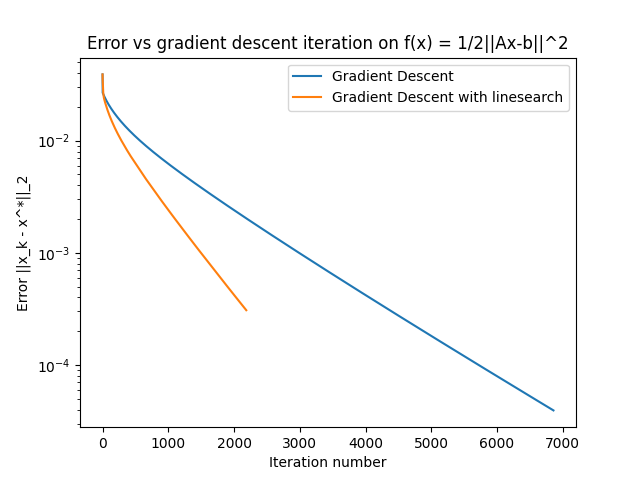
\includegraphics[width=0.6\linewidth]{Images/gradient_descent_results.png}
    \captionof{figure}{Gradient Descent (with and without linesearch) on a random 100x50 least-squares problem}
    \label{fig:grad-descent-err}
\end{center}

\section{Problem 3}
For sake of simplicity, we copy-and-pasted \footnote{Certainly, code could and should be reused in a professional implementation}
the gradient descent code from the previous problem and replaced the line which assigns to the $x\_1$ variable with the code
shown in figure \ref{fig:linesearch-code}.

The plot in figure \ref{fig:grad-descent-err} shows that the first-order algorithm converges to the same $x^*$ least-squares
solution with and without the linesearch component. Interestingly, the linesearch converges in fewer iterations, but the inter-iteration
tolerance condition causes the algorithm to terminate early.


\begin{center}
    \begin{python}

def descent_with_search(f, grad, x0, c=1e-4, rho=0.9, t0=1e-3, tol=1e-6, maxiters=int(1e3)):
    # ... initialize
    t = t0
    # ...begin iteration
        # Replace x1 assignment with linesearch algorithm:
        p = -grad(x0)
        norm2_p = np.vdot(p, p)
        while f(x0 + t * p) > f0 - c * t * norm2_p:
            t *= rho
        x1 = x0 + t * p
        # ... skipping exit criteria
        # Double t at the end of the loop
        t *= 2
    \end{python}
    \captionof{figure}{Modifications to code in figure \ref{fig:grad-descent} to enable linesearch} 
    \label{fig:linesearch-code}
\end{center}

\section{Problem 4}

\begin{enumerate}
\item Code which implements the vectorized gradient method is shown in figure \ref{fig:grad-code2}.
It runs very quickly at 0.2ms/call over a 1000 calls (see code in figure \ref{fig:timing} in the Appendix).
The code also continues to pass the visual gradient check from Problem 1.

\item We try running both the gradient descent as well as the gradient-descent with line search algorithms.
Code is shown in figure \ref{fig:training-code}. Figure \ref{fig:cost-eval}
contains a plot of function evaluation vs iteration. For some reason, the
function evaluation does not converge to something reasonable. We also have an overflow warning that the code
is raising during the function evaluation. This signals something is likely incorrect.

\item Indeed, using the code in figure \ref{fig:classify}, we find a misclassification
rate of around 40\%, even on the training data.
Clearly, something is causing the convergence rate to decay prematurely. Potentially related to the aforementioned
overflow error. Unfortunately, I ran out of time to debug this one.



\begin{center}
    \begin{python}
class LogLikelihoodLogistic:
    X: np.ndarray  # shape NxP where N is number of data points
    y: np.ndarray # shape N vector of labels

    def __init__(self, X, y):
        self.N, self.P = X.shape
        self.y = np.asarray(y)
        assert self.y.shape[0] == self.N
        self.X = X

    def mu(self, w):
        # print('w', w.shape)
        return sigmoid(self.y * (self.X @ w))

    def grad(self, w):
        # print(self.X.T.shape)
        # print(self.y.shape)
        # print(self.mu(w).shape)
        return - self.X.T @ (self.y * (1 - self.mu(w)))
    \end{python}
    \captionof{figure}{Vectorized gradient code}
    \label{fig:grad-code2}

\end{center}

\begin{center}
\begin{python}
def train(X, y):
    w0 = np.zeros(X.shape[1])
    ell = LogLikelihoodLogistic(X, y)
    return descent_with_search(ell.f, ell.grad, w0, t0=1e-2, maxiters=10000)
    # return gradient_descent(ell.f, ell.grad, w0, stepsize=1e-8, maxiters=10000)

res = train(X[:N_train], y[:N_train])
\end{python}
    \captionof{figure}{Training code}
    \label{fig:training-code}
\end{center}

\begin{center}
    
\includegraphics{Images/cost_eval.png}
    \captionof{figure}{Cost vs. iteration}
    \label{fig:cost-eval}
\end{center}

\begin{center}
    \begin{python}
ell_train = LL(X[:N_train], y[:N_train])
ell_test = LL(X[N_train:], y[N_train:])

def classify(ell, sol):
    prob = sigmoid(X[:N_train] @ w)
    return np.where(prob > 0.5, 1, -1)

class_train = classify(ell_train, res.solution)
misclass_train = np.sum(class_train != y[N_train])
print(misclass_train / N_train)

>>> 0.401305057096248
    \end{python}
    \captionof{figure}{(Mis)classification code for training data}
    \label{fig:classify}
\end{center}

\end{enumerate}









\appendix
\section{Code for Problem 1}
\label{sec:A1}

\begin{center}
\begin{python}
import numpy as np
from dataclasses import dataclass
import matplotlib.pyplot as plt
import cvx_opt.functions as funcs


def std_basis(n, i):
    # Return i-th standard basis vector.
    out = np.zeros(n)
    out[i] = 1
    return out

def _grad_central_diff(f, x0, h):
    n = x0.shape[0]
    return np.array([
        (f(x0 + h * std_basis(n, i)) - f(x0 - h * std_basis(n, i))) / (2*h)
        for i in range(n)
    ])
    
def _grad_finite_diff(f, x0, h):
    n = x0.shape[0]
    f0 = f(x0)
    return np.array([
        (f(x0 + h * std_basis(n, i)) - f0) / h
        for i in range(n)
    ])
    

METHODS = {
    'central': _grad_central_diff,
    'finite_diff': _grad_finite_diff,
}
    

def grad(f, x0, h, method=None):
    if method not in METHODS:
        raise ValueError(f"Unknown method: '{method}'. Must be one of {METHODS.keys()}")
    return METHODS[method](f, x0, h)
    

@dataclass
class ErrorInfo:
    # Stepsizes
    h: np.ndarray
    x0: np.ndarray
    # RMS Error in numeric versus
    # ||grad_numeric(f, x0, h) - grad_analytic(f, x0)||_2
    errors_by_method: dict


def test_gradient(f, grad_f, x0):
    # Check whether that the given analytic gradient grad_f is 
    # close to the gradient computed numerically from f at a given
    # point x0.
    h = np.logspace(0, -15, 31)
    all_errors = {}
    for method in METHODS.keys():
        errors = np.full_like(h, np.nan)
        for i, h_i in enumerate(h):
            numeric_grad = grad(f, x0, h_i, method)
            analytic_grad = grad_f(x0)
            errors[i] = np.linalg.norm(numeric_grad - analytic_grad)
        all_errors[method] = errors

    
    return ErrorInfo(h=h, x0=x0, errors_by_method=all_errors)


def plot_errors(info, func_name, save_dir):
    fig = plt.figure()
    for method, error in info.errors_by_method.items():
        plt.loglog(info.h, error, '-o', label=method)
    plt.legend()
    plt.xlabel("h (stepsize)")
    plt.ylabel("error")
    plt.title(f"Numeric gradient error for {func_name} \n at {np.round(info.x0, 2)}")
    x0_str = np.round(info.x0, 2)[0]
    filename = f"{x0_str}_{func_name.replace(' ', '_')}.png"
    print(filename)
    fig.savefig(save_dir / filename)
        
        
        

def problem_1(save_dir=None):
    np.random.seed(0)
    N = 10
    P = 5
    X = np.random.uniform(0, 10, (N, P))
    y = np.where(np.random.uniform(0, 1, N) < 0.5, -1, 1)
    w0_log = np.random.uniform(-5, 5, P)


    x0_1d = np.array([5])
    for x0, func in [
        (x0_1d, funcs.Quadratic(5, 1, 20)),
        (x0_1d, funcs.Linear(21.0, 5.)),
        (x0_1d, funcs.Cubic([5, 4, 3, 2])),
        (w0_log, funcs.LogLikelihoodLogistic(X, y)),
        (np.zeros(P), funcs.LogLikelihoodLogistic(X, y))
    ]:
        e = test_gradient(func.f, func.grad, x0)
        plot_errors(e, str(func), save_dir)
                        
\end{python}
    \label{fig:python1}
    \captionof{figure}{Gradient Checking Code}
\end{center}

\begin{center}
\begin{python}
import numpy as np
from dataclasses import dataclass


@dataclass
class Linear:
    a: float
    b: float

    def f(self, x):
        return self.a * x + self.b

    def grad(self, x):
        return self.a

@dataclass
class Affine:
    A: np.ndarray
    b: np.ndarray
    
    def f(self, x):
        return self.A @ x + self.b
        
    def grad(self, x):
        return self.A

@dataclass
class Quadratic:
    a: float
    b: float
    c: float 
    def f(self, x):
        return self.a * x**2 + self.b * x + self.c

    def grad(self, x):
        return 2 * self.a * x + self.b

@dataclass
class Cubic:
    c: np.ndarray
    
    def __init__(self, c):
        self.c = np.asarray(c)
        assert self.c.shape[0] == 4
        
    def f(self, x):
        return np.vdot(self.c, np.r_[x**3, x**2, x, 1])

    def grad(self, x):
        return np.vdot(self.c[:-1], np.r_[3 * x**2, 2*x, 1])


def sigmoid(a):
    return 1 / (1 + np.exp(-a))
    
class LogLikelihoodLogistic:
    X: np.ndarray  # shape NxP where N is number of data points
    y: np.ndarray # shape N vector of labels

    def __init__(self, X, y):
        self.N, self.P = X.shape
        self.y = np.asarray(y)
        assert self.y.shape[0] == self.N
        self.X = X

    def alpha(self, i, w):
        return -self.y[i] * np.vdot(w, self.X[i])
        
    def f(self, w):
        return np.sum(
            [np.log1p(np.exp(self.alpha(i, w)))
             for i in range(self.N)]
        )

    def grad(self, w):
        return -np.sum(
            [sigmoid(self.alpha(i, w)) * self.y[i] * self.X[i]
             for i in range(self.N)], axis=0)

    def __repr__(self):
        return f"Logistic(X.shape={self.X.shape}, y.shape={self.y.shape}"
\end{python}
    \label{fig:python2}
    \captionof{figure}{Functions with known gradients}
\end{center}

\section{Problem 4 Additional code}

\begin{center}
    \begin{python}
# Data loading and transformation
data = np.loadtxt(DATA_DIR / 'spam.data', delimiter=" ")
X, y = data[:, :-1], data[:, -1]
y[y==0] = -1
X = shuffle(X)
X = np.log(X + 0.1)
X = shuffle(X)

import time

def timeit(f, n_times=int(1e3)):
    ts = []
    for i in range(n_times):
        t = time.monotonic()
        f()
        ts.append(time.monotonic() - t)
    print('Average time: ', np.mean(ts))

ell = LogLikelihoodLogistic(X, y)
w0 = np.zeros(X.shape[1])
print("w=0")
timeit(lambda: ell.grad(w0))

>>> 0.00020956742367707194
    \end{python}
    \captionof{figure}{Data loading and timing code for problem 4a}
    \label{fig:timing}
\end{center}

\end{document}
